\chapter{Implementacija i korisničko sučelje}
		
		
		\section{Korištene tehnologije i alati}
		
			Komunikacija unutar tima realizirana je korištenjem aplikacija \underline{WhatsApp}\footnote{\url{https://www.whatsapp.com/}} i \underline{Discord}\footnote{\url{https://discord.com/}}. Za izradu UML dijagrama korišten je alat \underline{Astah Professional}\footnote{\url{https://astah.net/}}. Kao sustav za upravljanje izvornim kodom upotrebljavali smo \underline{Git}\footnote{\url{https://git-scm.com/}}, a udaljeni repozitorij projekta je dostupan na web platformi \underline{GitHub}\footnote{\url{https://github.com/}}.

			Kao razvojna okruženja korišteni su \underline{Android Studio}\footnote{\url{https://developer.android.com/studio}} i \underline{PyCharm}\footnote{\url{https://www.jetbrains.com/pycharm/}}. Android Studio je integrirano razvojno okruženje za Googleov operativni sustav Android, izgrađeno na JetBrainsovom IntelliJ IDEA softveru i dizajnirano posebno za Android razvoj. Dostupan je za preuzimanje na Windows, macOS i Linux operativnim sustavima. PyCharm  je integrirano razvojno okruženje koje se koristi za programiranje u Pythonu koji je razvila tvrtka JetBrains. Omogućuje analizu koda, integrirani tester jedinica \textit{(engl. unit testing)}, grafički \textit{debugger} i podržava web razvoj s Djangom. Isto kao i Android Studio, dostupan je na različitim operacijskim sustavima.

			Aplikacija je napisana koristeći radni okvir \underline{FastAPI}\footnote{\url{https://fastapi.tiangolo.com/}} i jezik \underline{Python}\footnote{\url{https://www.python.org/}} za izradu \textit{backenda} te jezik \underline{Kotlin}\footnote{\url{https://kotlinlang.org/}} za izradu \textit{frontenda}. FastAPI je moderan web okvir za izgradnju RESTful API-ja u Pythonu. Popularan je među programerima zbog svoje jednostavnosti, robusnosti i brzine.

			Baza podataka se nalazi na poslužitelju u \underline{Renderu}\footnote{\url{https://render.com/}}. To je objedinjeni oblak za izradu i pokretanje svih aplikacija i web stranica s besplatnim TLS certifikatima, globalnim CDN-om, privatnim mrežama i automatskim deploymentom iz Gita.
			
			\eject 
		
	
		\section{Ispitivanje programskog rješenja}
			
			Ispitivanje aplikacije provelo se na strukturiran način pomoću unit testova na \textit{backendu} i ručno na \textit{frontendu} zato što se preporučeni Selenium testovi koriste za web, a ne i za mobilne aplikacije. Aplikaciju smo ispitali po obrascima uporabe kako bi provjerili svu osnovnu funkcionalnost aplikacije, kao i nasumičnim kretanjem po aplikaciji kako bi otkrili moguća nepredviđena ponašanja i ispravili neočekivane greške. Ispitan je cijeli sustav, no zbog jednostavnosti dokumentacije ovdje će biti prikazan samo dio testova.
			
			\subsection{Ispitivanje komponenti}
		
			Proveli smo ispitivanje jedinica (engl. \textit{unit testing}) nad razredima koji implementiraju osnovne funkcionalnosti. U nastavku će biti prikazan izvorni kod i prikaz rezultata izvođenja ispita u razvojnom okruženju.

			Za konfiguraciju i provođenje svih testova bile su nam potrebne sljedeće funkcije: 
	
			\begin{packed_item}
			
				\item pytest{\_}configure - stvara testnu bazu na lokalnom poslužitelju prije testiranja
				\item pytest{\_}unconfigure - \textit{dropa} lokalnu tekstnu bazu nakon završetka testiranja
				\item pytest fixture test{\_}session - da testovi nebi utjecali jedan na drugog, za svakog stvori izoliranu okolinu
				\item mock{\_}user{\_}token - dependency override za provjeru tokena na endpointima, token se provjerava zasebno
				\item user{\_}factory - direktno stvara usera na bazi
				\item advert{\_}factory - direktno stvara advert na bazi
			
			\end{packed_item}

			Izvorni kod navedenih funkcija priložen je u nastavku.
			\begin{lstlisting}[language=Python]
def pytest_configure():
    create_database(
        URL.create(
            "postgresql",
            username=settings.POSTGRES_USER,
            password=settings.POSTGRES_PASSWORD,
            host=settings.POSTGRES_HOST,
            port=settings.POSTGRES_PORT,
            database=settings.TEST_DATABASE,
        )
    )

def pytest_unconfigure():
    drop_database(
        URL.create(
            "postgresql",
            username=settings.POSTGRES_USER,
            password=settings.POSTGRES_PASSWORD,
            host=settings.POSTGRES_HOST,
            port=settings.POSTGRES_PORT,
            database=settings.TEST_DATABASE,
        )
    )

@pytest.fixture(scope="function")
def test_session():
    EngineManager.set_database(settings.TEST_DATABASE)
    engine = EngineManager.get_engine()
    Base.metadata.create_all(engine)

    test_session_mold = sessionmaker(bind=engine, expire_on_commit=False)
    test_session = test_session_mold()
    yield test_session

    Base.metadata.drop_all(engine)
    EngineManager.unset_database()

def mock_user_token():
    return 1

def user_factory(user_id: int, session: Session):
    user = (
        UserCustom(
                id=user_id,
                username=('test_username_' + str(user_id)),
                is_shelter=False,
                email='test_email',
                phone_number='test_number'
        )
    )
    user_auth = UserAuth(username=('test_username_' + str(user_id)), password='1234')
    session.add(user)
    session.add(user_auth)
    session.commit()
    return user

def advert_factory(id: int, user_id: int, session: Session):
    pet = Pet(
        id=id,
        name=('test_pet_' + str(id)),
        location_lost=('test_location_' + str(id)),
    )
    advert = Advertisement(
        id=id,
        pet_id=id,
        user_id=user_id,
        category='lost'
    )
    session.add(pet)
    session.add(advert)
    session.commit()
			\end{lstlisting}

			U nastavku je naveden dio testova koje smo proveli.

			Klasa \textit{TestAuthentication} provodi dva testa. Prvi test ispitao je generiranje i dekodiranje korisničkog tokena. Drugi test ispitao je funkcionalnost prijave i registracije korisnika pri ulasku u aplikaciju. Komponenta je prošla testove i rezultat ispitivanja prikazan je na slici \ref{fig:test1i2}. Izvorni kod za ova dva testa je sljedeći: 
			\begin{lstlisting}
class TestAuthentication:

    def test_auth_utils(self, test_session):
        user = user_factory(1, test_session)
        token = generate_token(user)
        assert len(token) == 181

        decoded = validate_token(token)
        assert decoded == user.id

    def test_signup_and_login(self, test_session):
        with TestClient(app) as client:
            result_signup = client.post(
                "/api/authorization/signup",
                json={
                    "username": "test_shelter",
                    "password": "password",
                    "is_shelter": True,
                    "shelter_name": "Test Shelter",
                    "email": "test@shelter.com",
                    "phone_number": "111"
                }
            )

            assert result_signup.status_code == 201
            assert result_signup.json().get("detail") == "User successfully saved"

            result_login = client.post(
                "/api/authorization/login",
                json={
                    "username": "test_shelter",
                    "password": "password"
                }
            )

            assert result_login.status_code == 200
            assert result_login.json().get("token") is not None
            assert result_login.json().get("is_shelter")
            assert result_login.json().get("current_user_username") == "test_shelter"
			\end{lstlisting}

			\begin{figure}[H]
			 	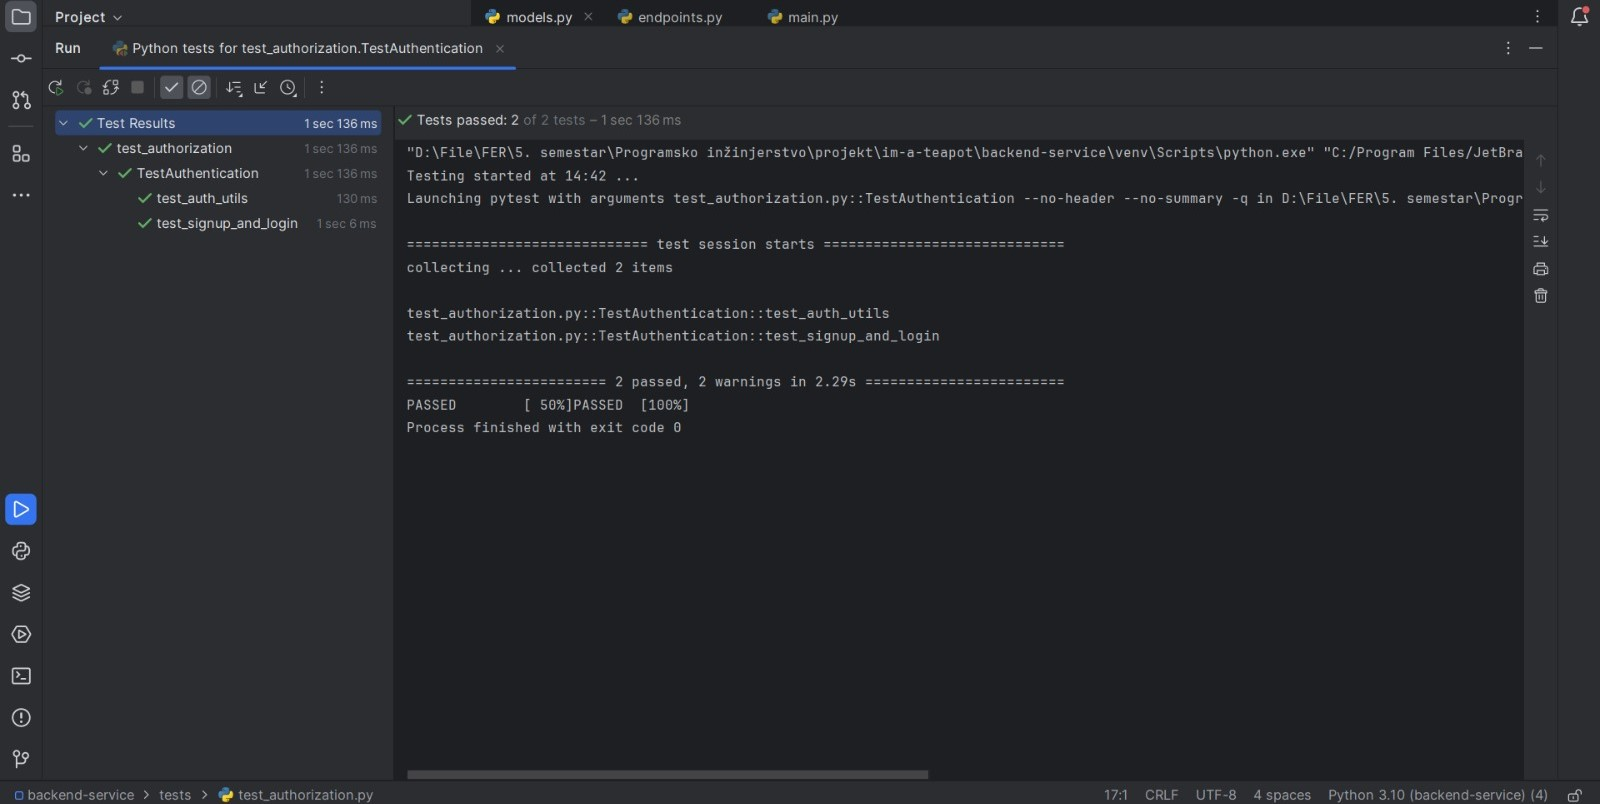
\includegraphics[scale=0.42]{slike/test1i2.jpg} %veličina slike u odnosu na originalnu datoteku i pozicija slike
			 	\centering
			 	\caption{Rezultati testa 1. i testa 2.}
			 	\label{fig:test1i2}
			 \end{figure}

			Klasa \textit{TestMessaging} provjerava slanje i dohvaćanje poruka o nestalom ljubimcu. Komponenta je prošla test i rezultat ispitivanja prikazan je na slici \ref{fig:test3}. Izvorni kod testa je sljedeći:
			\begin{lstlisting}
class TestMessaging:

    def test_add_and_fetch_message(self, test_session):
        app.dependency_overrides[validate_token] = mock_user_token
        user_factory(1, test_session)
        user_factory(2, test_session)
        advert_factory(1, 1, test_session)

        with TestClient(app) as client:
            result = client.post(
                "/api/messages/1/add",
                json={
                    "text": "message_1"
                }
            )
            assert result.status_code == 200

            client.post(
                "/api/messages/1/add",
                json={
                    "text": "message_2"
                }
            )
            assert result.status_code == 200

            result = client.get(
                "/api/messages/1"
            )
            assert result.status_code == 200
            assert len(result.json()) == 2
			\end{lstlisting}

			\begin{figure}[H]
			 	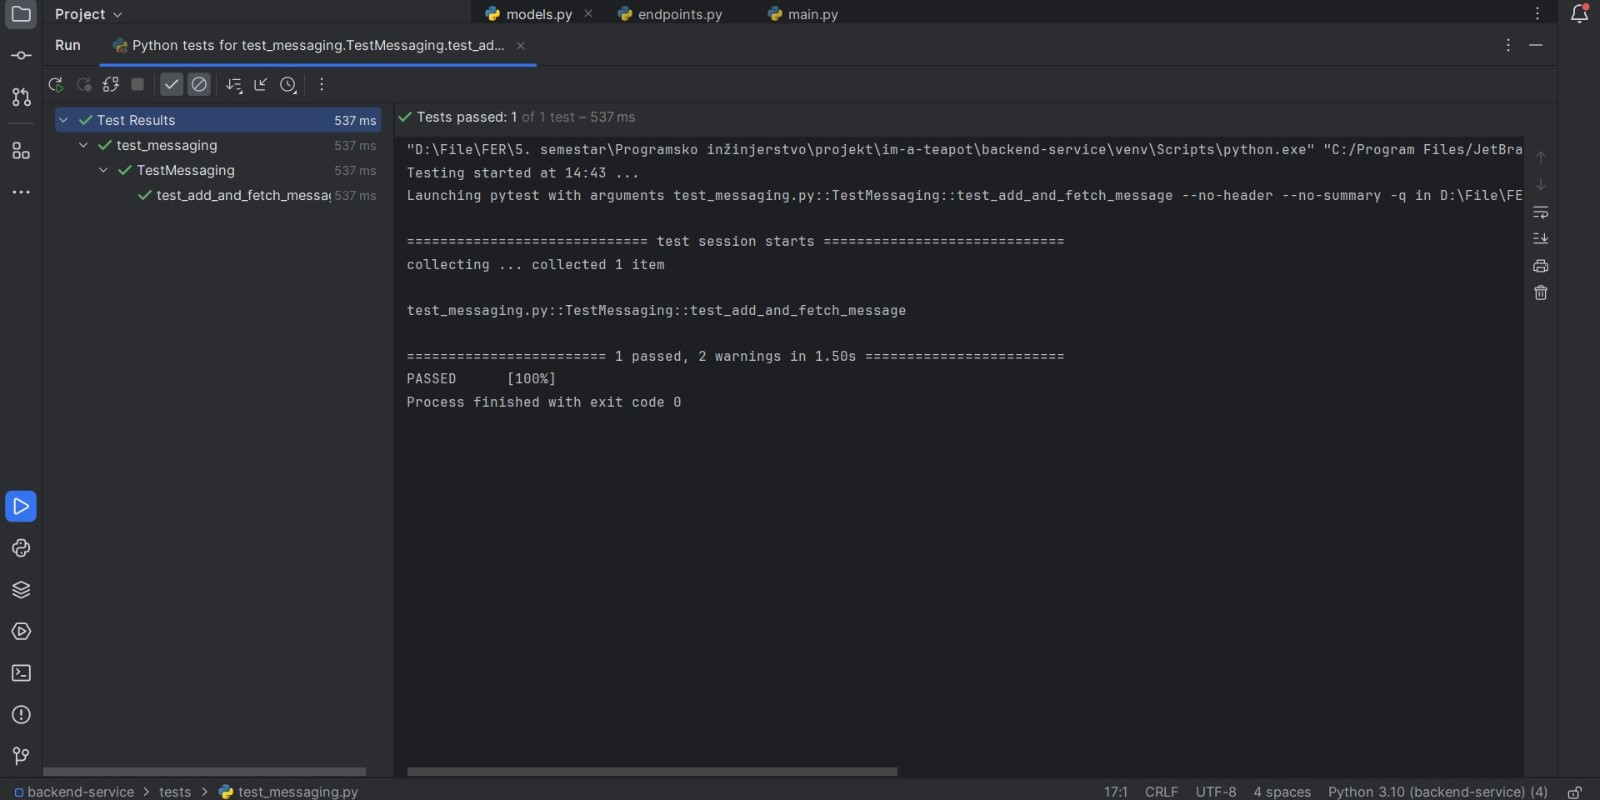
\includegraphics[scale=0.42]{slike/test3.jpg} %veličina slike u odnosu na originalnu datoteku i pozicija slike
			 	\centering
			 	\caption{Rezultati testa 3.}
			 	\label{fig:test3}
			 \end{figure}

			Klasa \textit{TestAdvertActions} izvodi tri testa nad oglasima o nestalim ljubimcima. Ispitala je postavljanje, izmjenu i brisanje oglasa. Komponenta aplikacije je prošla sva tri testa i rezultati su prikazani na slici \ref{fig:test4i5i6}. Izvorni kod ovih testova je sljedeći:
			\begin{lstlisting}
class TestAdvertActions:

    def test_create(self, test_session):
        app.dependency_overrides[validate_token] = mock_user_token
        user_factory(1, test_session)
        with TestClient(app) as client:
            result = client.post(
                "/api/advert/create",
                json={
                    "pet_name": "Edgar",
                }
            )
            assert result.status_code == 200

    def test_edit(self, test_session):
        app.dependency_overrides[validate_token] = mock_user_token
        user_factory(1, test_session)
        advert_factory(1, 1, test_session)
        with TestClient(app) as client:
            result = client.put(
                "/api/advert/1/edit",
                json={
                    "pet_name": "Allan",
                }
            )
            assert result.status_code == 200
            assert result.json().get("pet_name") == "Allan"

    def test_delete(self, test_session):
        app.dependency_overrides[validate_token] = mock_user_token
        user_factory(1, test_session)
        advert_factory(1, 1, test_session)
        with TestClient(app) as client:
            result = client.delete(
                "/api/advert/1/delete"
            )
            assert result.status_code == 200
			\end{lstlisting}

			\begin{figure}[H]
			 	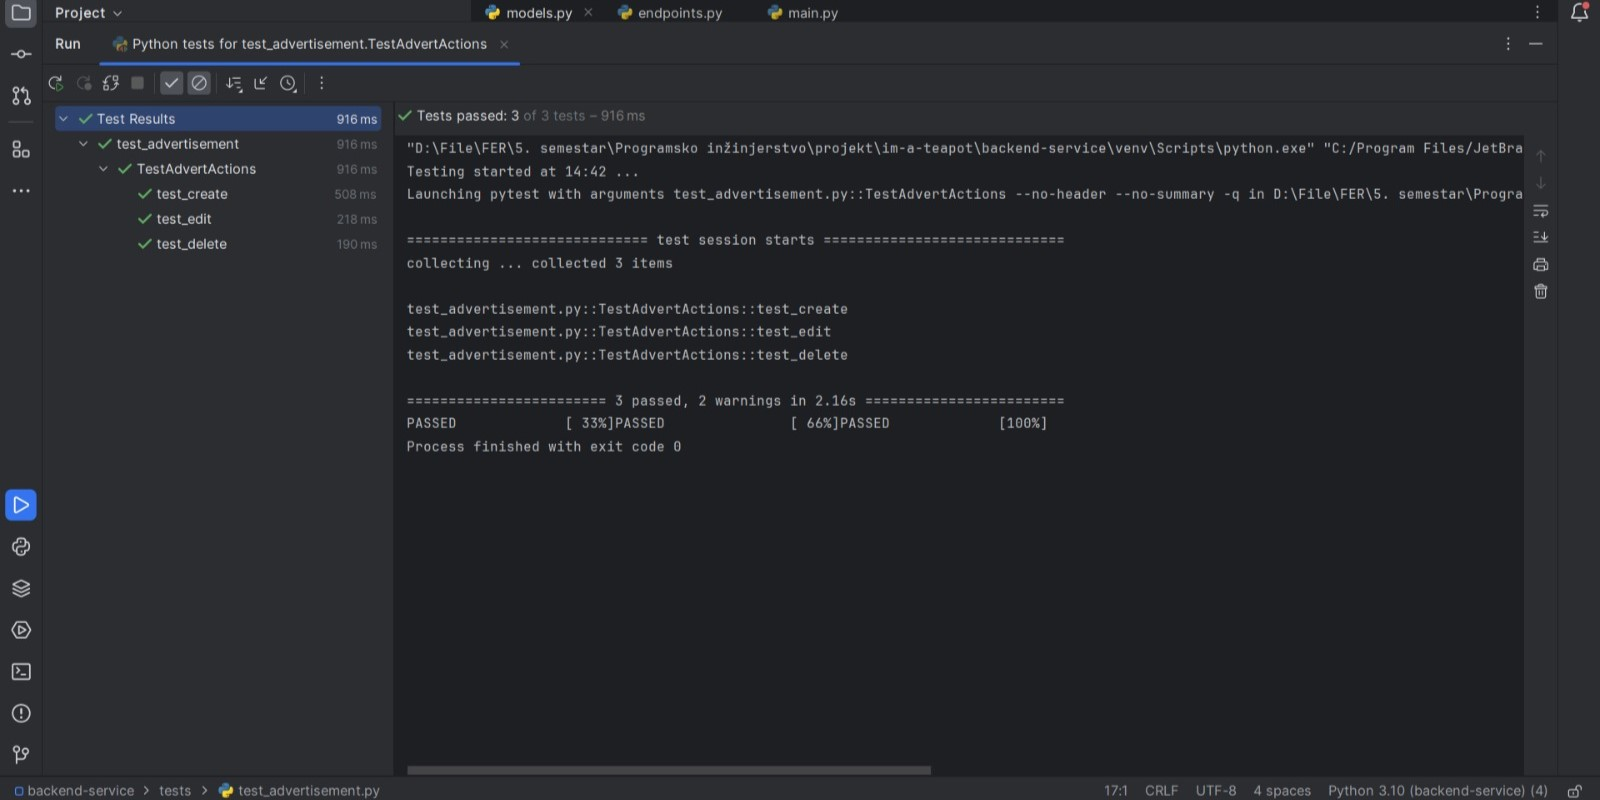
\includegraphics[scale=0.42]{slike/test4i5i6.jpg} %veličina slike u odnosu na originalnu datoteku i pozicija slike
			 	\centering
			 	\caption{Rezultati testa 4., testa 5. i testa 6.}
			 	\label{fig:test4i5i6}
			 \end{figure}

			Klasa \textit{TestHome} provodi dva testa. Prvi je ispitivanje pretraživanja po imenu ljubimca i po korisničkom imenu. Komponenta je prošla ovaj test, a rezultat ispitivanja prikazan je na slici \ref{fig:test7}. Druga stvar koju ova klasa ispituje je pretraživanje po lokaciji. Ta funkcionalnost nije implementirana u našoj aplikaciji, pa zato komponenta pada na ovom testu. Rezultat je prikazan na slikama \ref{fig:test8a} i \ref{fig:test8b}. Izvorni kod klase koja provodi ova ispitivanja prikazan je u nastavku.
			\begin{lstlisting}
class TestHome:

    def test_filter__by_pet_name_and_username(self, test_session):
        user_factory(1, test_session)
        user_factory(2, test_session)
        advert_factory(1, 1, test_session)
        advert_factory(2, 2, test_session)

        with TestClient(app) as client:
            result = client.get(
                "/api/advert/",
                params={"pet_name": "test_pet_1", "username": "test_username_1"}
            )

            assert result.status_code == 200
            assert len(result.json()) == 1

    def test_filter__by_location(self, test_session):
        user_factory(1, test_session)
        user_factory(2, test_session)
        advert_factory(1, 1, test_session)
        advert_factory(2, 2, test_session)

        with TestClient(app) as client:
            result = client.get(
                "/api/advert/",
                params={"location_lost": "test_location_1"}
            )

            assert result.status_code == 200
            assert len(result.json()) == 1
			\end{lstlisting}

			\begin{figure}[H]
			 	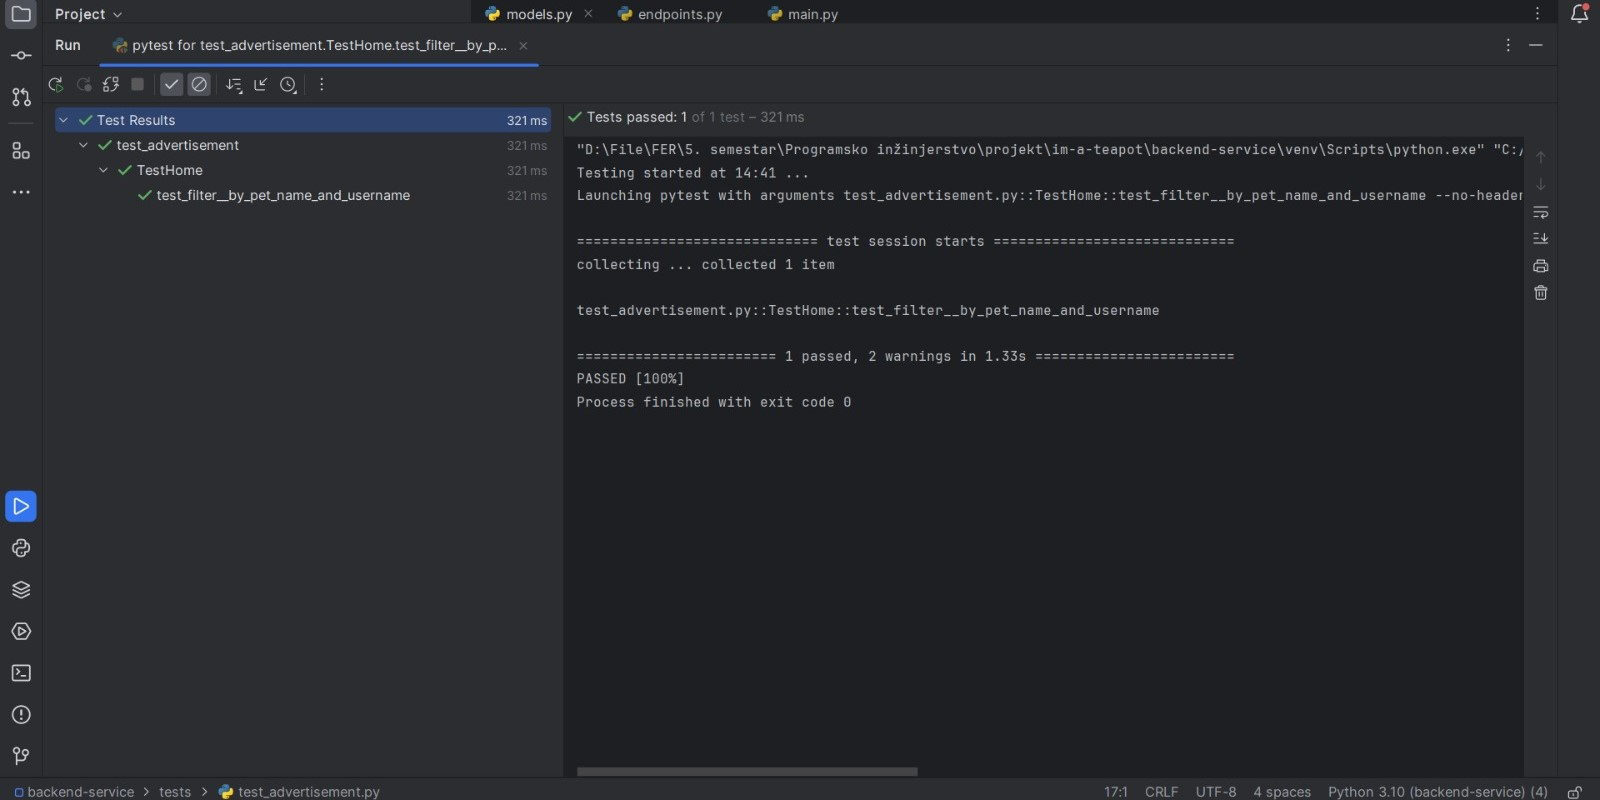
\includegraphics[scale=0.42]{slike/test7.jpg} %veličina slike u odnosu na originalnu datoteku i pozicija slike
			 	\centering
			 	\caption{Rezultati testa 7.}
			 	\label{fig:test7}
			 \end{figure}

			\begin{figure}[H]
			 	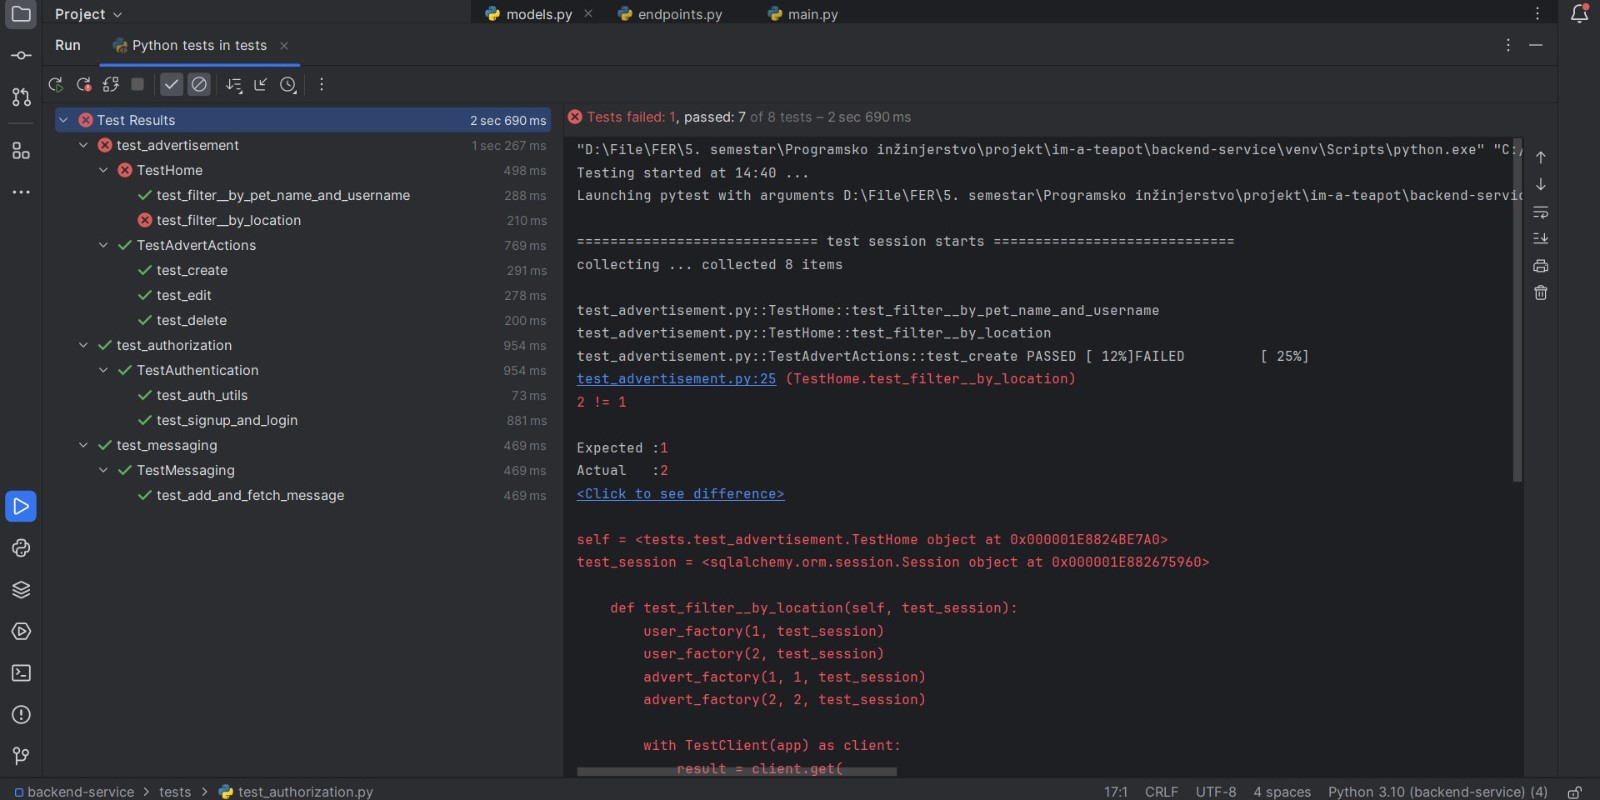
\includegraphics[scale=0.42]{slike/test8a.jpg} %veličina slike u odnosu na originalnu datoteku i pozicija slike
			 	\centering
			 	\caption{Rezultati testa 8. - 1. dio}
			 	\label{fig:test8a}
			 \end{figure}

			\begin{figure}[H]
			 	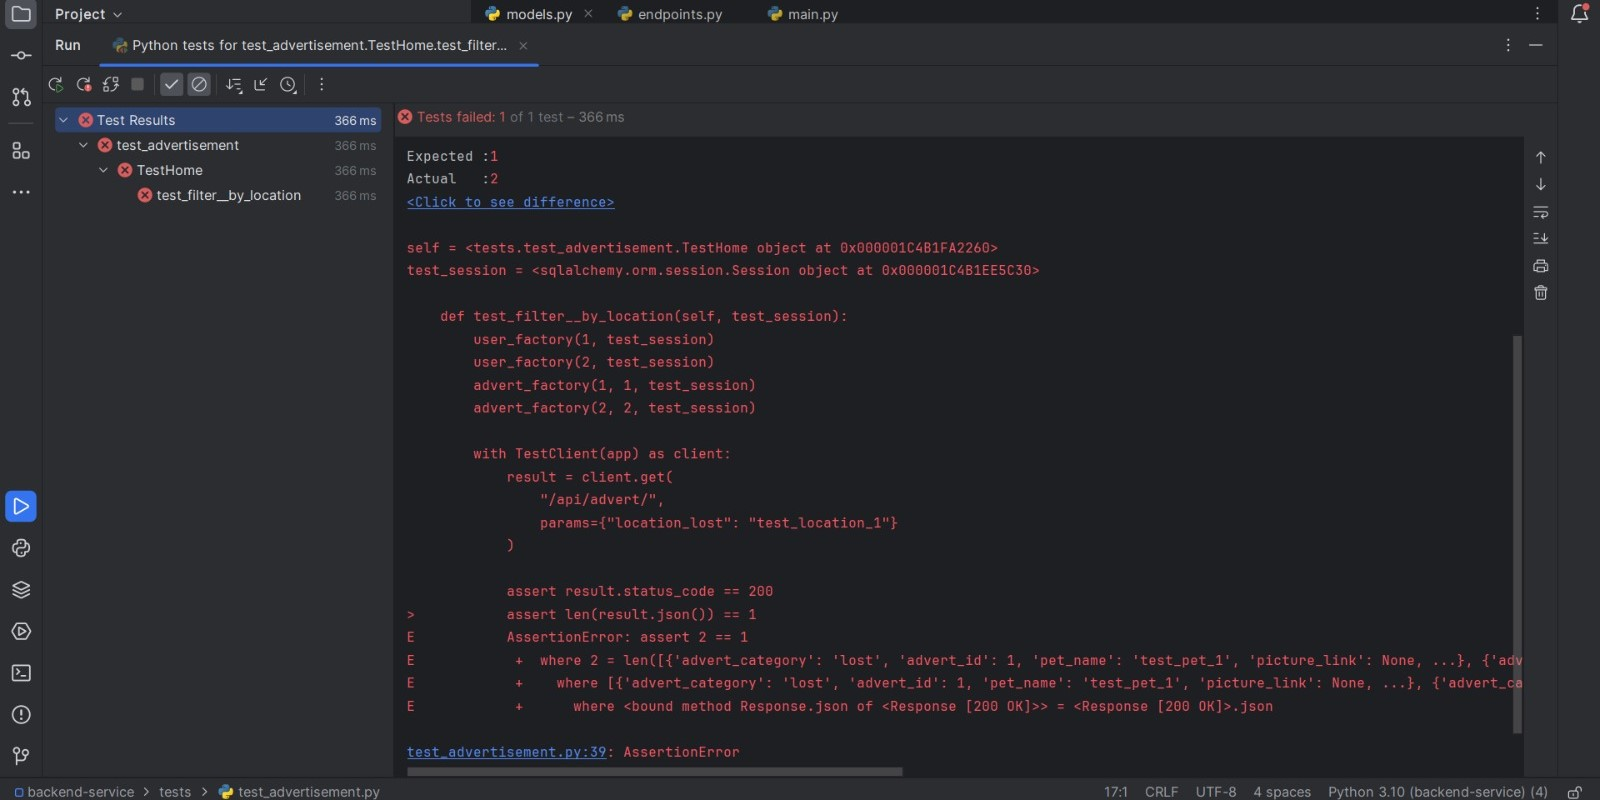
\includegraphics[scale=0.42]{slike/test8b.jpg} %veličina slike u odnosu na originalnu datoteku i pozicija slike
			 	\centering
			 	\caption{Rezultati testa 8. - 2. dio}
			 	\label{fig:test8b}
			 \end{figure}
			
			\subsection{Ispitivanje sustava}
			
			Ispitivanje sustava provedeno je ručno za sve obrasce uporabe. U nastavku su prikazani rezultati ispitivanja za UC2 (s UC15), UC3 (uključujući UC8), UC6 i UC9.

			\noindent \textbf{Ispitni  slučaj 1: Prijava korisnika u sustav}

			\noindent \textbf{Ulaz: }
			\begin{packed_enum}
				\item Otvaranje stranice za prijavu.
				\item Unos korisničkog imena i lozinke.
				\item Pritisak na gumb za prijavu.
			\end{packed_enum}

			\noindent \textbf{Očekivani rezultat: }
			\begin{packed_enum}
				\item Prikazuje se lista oglasa
				\item Odabirom ikone korisnika u \textit{toolbar-u} mogu se pregledati podaci o korisniku			
			\end{packed_enum}

			\noindent \textbf{Rezultat:} Očekivanja su zadovoljena. Aplikacija je prošla test.

			\begin{figure}[H]
			\centering
			\begin{minipage}{.5\textwidth}
	 			 \centering
				  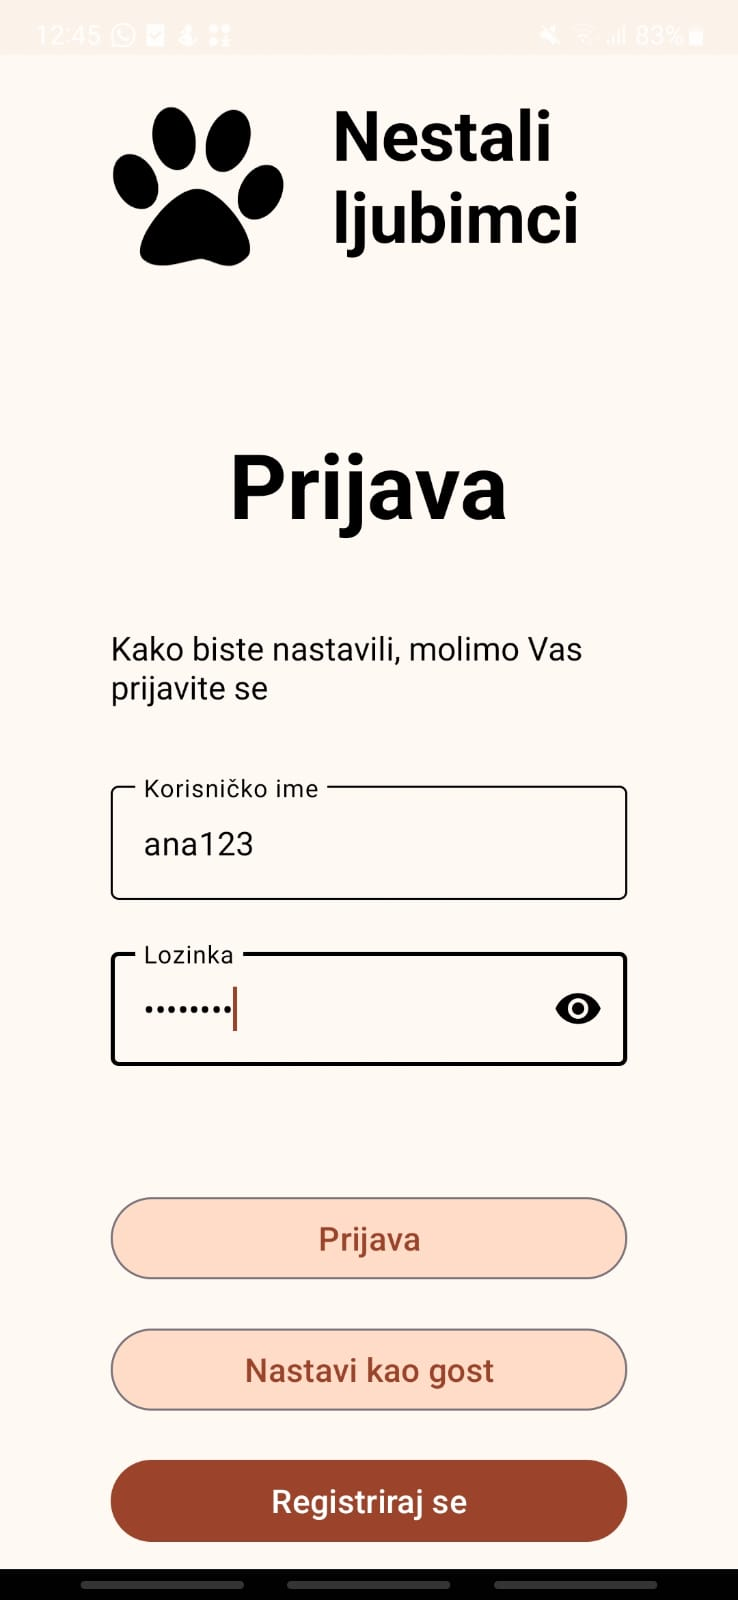
\includegraphics[width=.58\linewidth]{slike/app1v1.jpg}
				  \caption{Prijava u sustav}
				  \label{fig:app1v1}
			\end{minipage}%
			\begin{minipage}{.5\textwidth}
				  \centering
				  
\includegraphics[width=.58\linewidth]{slike/app1v2.jpg}
				  \caption{Prikaz profila}
				  \label{fig:app1v2}
			\end{minipage}
			\end{figure}

			\noindent \textbf{Ispitni  slučaj 2: Postavljanje oglasa}

			\noindent \textbf{Ulaz: }
			\begin{packed_enum}
				\item Odabir opcije "Dodaj oglas".
				\item Otvaranje forme za unos podataka.
				\item Unos podataka o nestalom ljubimcu.
				\item Pritisak na gumb za objavu oglasa.
			\end{packed_enum}

			\noindent \textbf{Očekivani rezultat: }
			\begin{packed_enum}
				\item[]\begin{packed_enum}
					\item	 Prikazuje se detaljni prikaz stvorenog oglasa.
					\item Nudi se mogućnost pisanja komentara.
				\end{packed_enum}	
			\end{packed_enum}

			\noindent \textbf{Rezultat:} Očekivanja su zadovoljena. Aplikacija je prošla test.

			\begin{figure}[H]
			\centering
			\begin{minipage}{.5\textwidth}
	 			 \centering
				  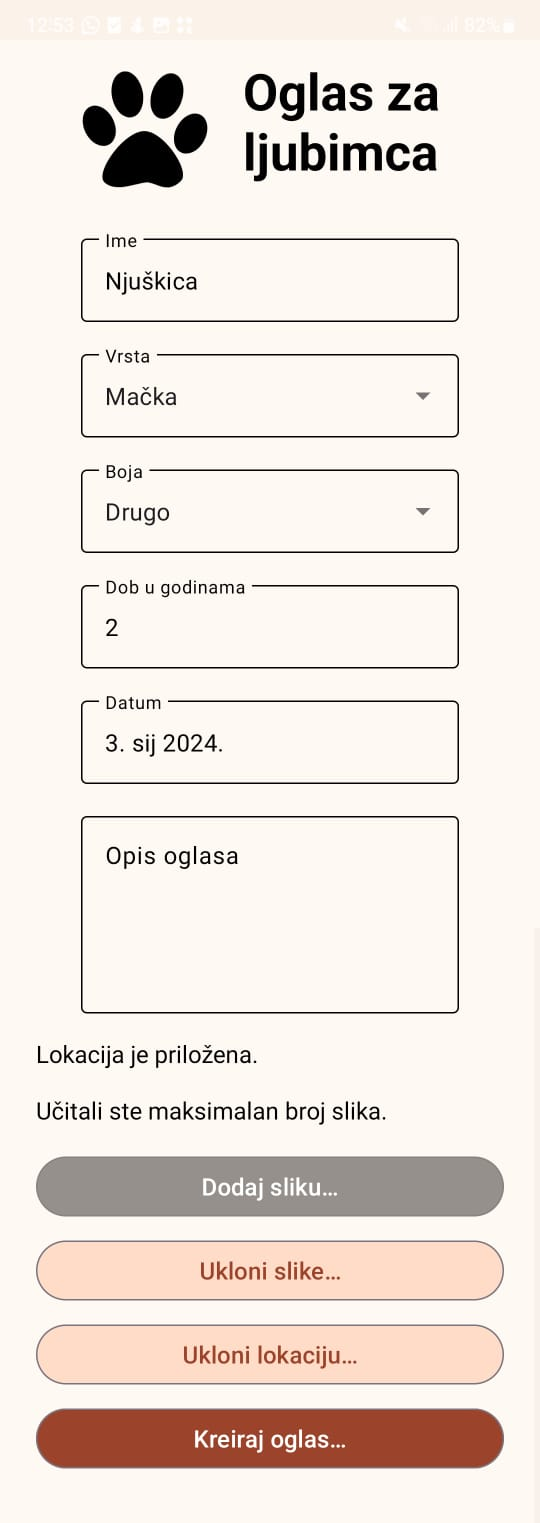
\includegraphics[width=.58\linewidth]{slike/app2v1.jpg}
				  \caption{Stvaranje novog oglasa}
				  \label{fig:app2v1}
			\end{minipage}%
			\begin{minipage}{.5\textwidth}
				  \centering
				  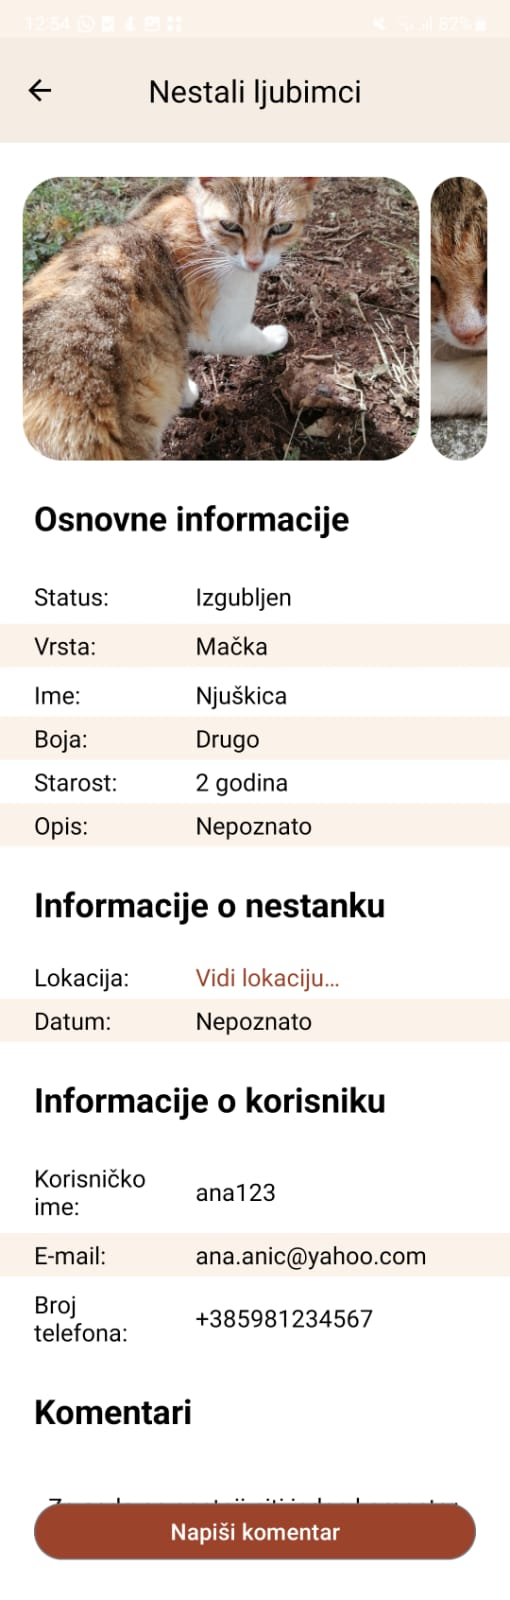
\includegraphics[width=.58\linewidth]{slike/app2v2.jpg}
				  \caption{Prikaz stvorenog oglasa}
				  \label{fig:app2v2}
			\end{minipage}
			\end{figure}

			\noindent \textbf{Ispitni  slučaj 3: Prikaz liste i pregled oglasa}

			\noindent \textbf{Ulaz: }
			\begin{packed_enum}
				\item Otvaranje aplikacije (već prijavljen korisnik ili odabir ulaska kao gost).
				\item Odabire se oglas za prikaz.
			\end{packed_enum}

			\noindent \textbf{Očekivani rezultat: }
			\begin{packed_enum}
				\item	 Prikazuje se lista svih oglasa.
				\item Prikazuje se detaljni prikaz odabranog oglasa.
			\end{packed_enum}

			\noindent \textbf{Rezultat:} Očekivanja su zadovoljena. Aplikacija je prošla test.

			\begin{figure}[H]
			\centering
			\begin{minipage}{.5\textwidth}
	 			 \centering
				  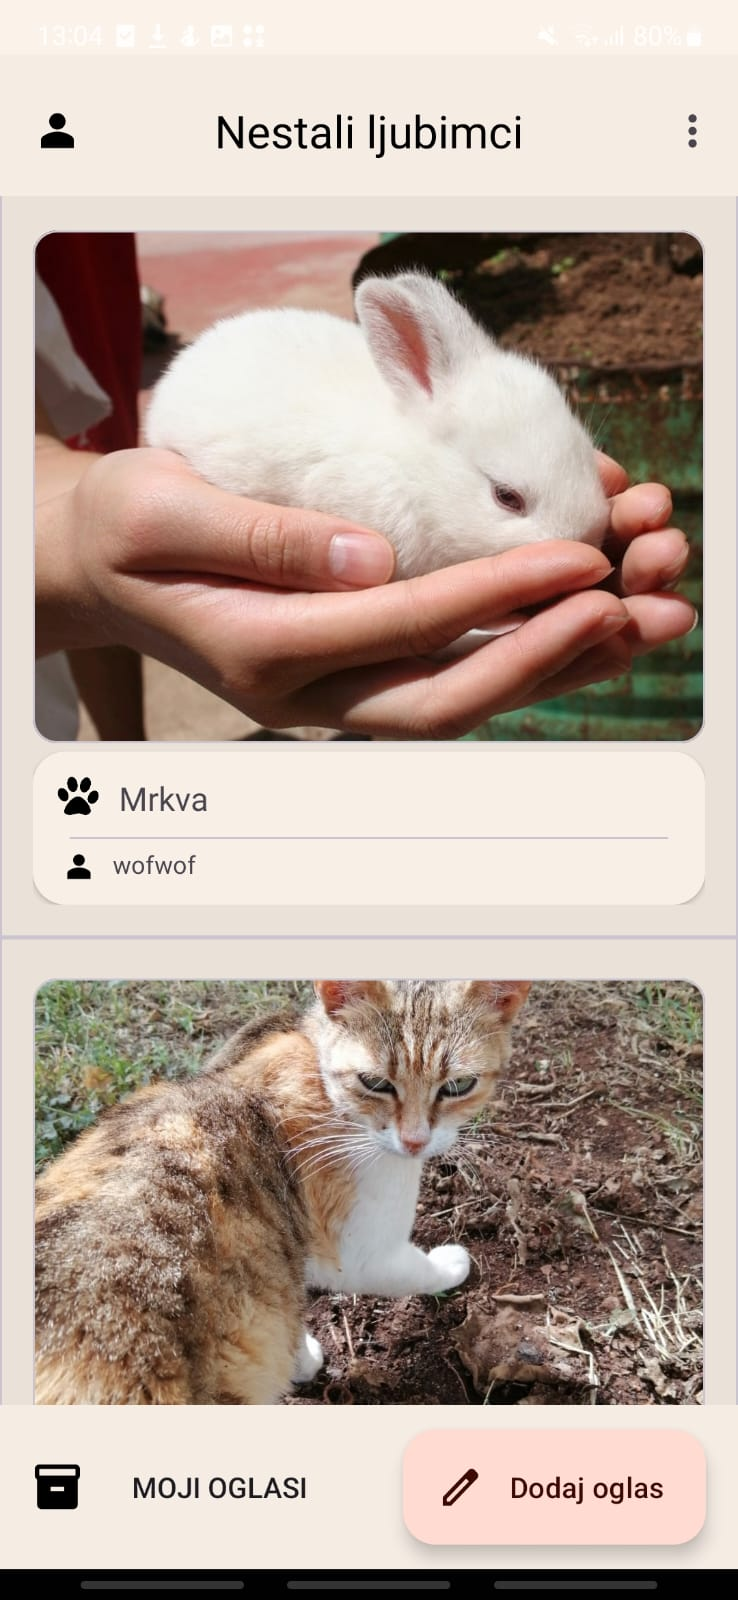
\includegraphics[width=.58\linewidth]{slike/app3v1.jpg}
				  \caption{Lista oglasa}
				  \label{fig:app3v1}
			\end{minipage}%
			\begin{minipage}{.5\textwidth}
				  \centering
				  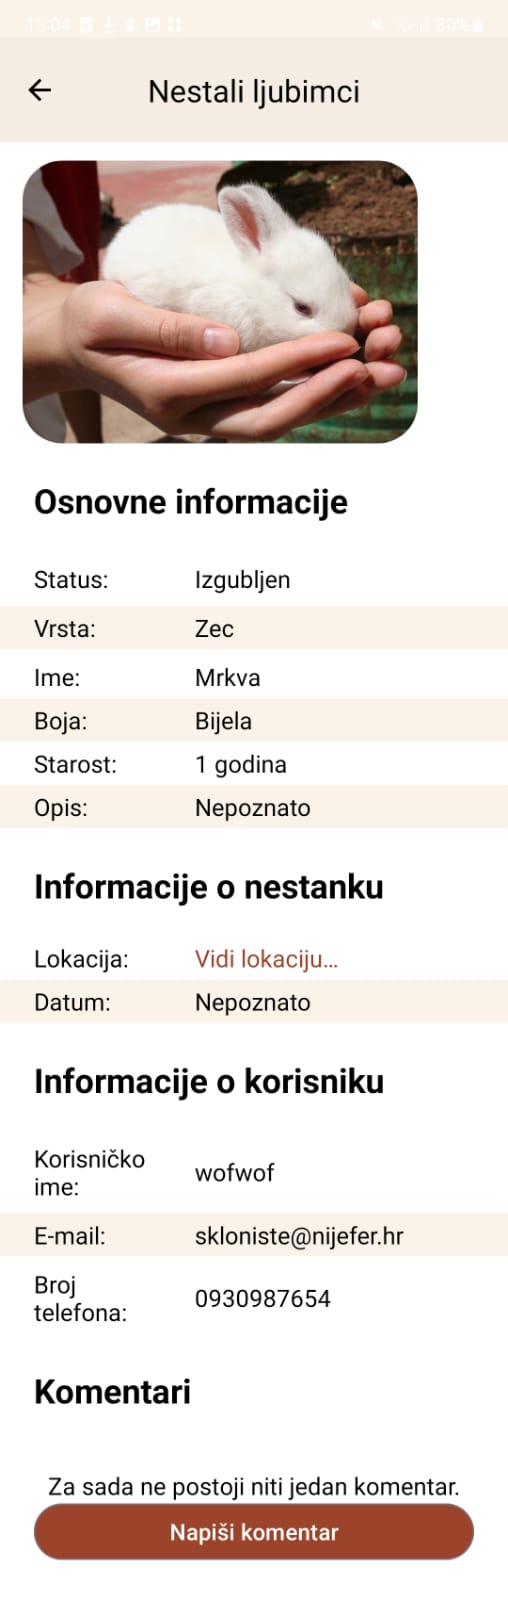
\includegraphics[width=.58\linewidth]{slike/app3v2.jpg}
				  \caption{Detaljni prikaz oglasa}
				  \label{fig:app3v2}
			\end{minipage}
			\end{figure}
			
			\noindent \textbf{Ispitni  slučaj 4: Brisanje oglasa}

			\noindent \textbf{Ulaz: }
			\begin{packed_enum}
				\item Pregled vlastitih oglasa.
				\item Odabir opcije za brisanje.
				\item Potvrda brisanja.
			\end{packed_enum}

			\noindent \textbf{Očekivani rezultat: }
			\begin{packed_enum}
				\item	[]\begin{packed_enum}
					\item	 Ispis poruke o uspješnom brisanju.
					\item Prikaz preostalih vlastitih oglasa ili poruka da ih više nema.
				\end{packed_enum}	
			\end{packed_enum}	

			\noindent \textbf{Rezultat:} Očekivanja su zadovoljena. Aplikacija je prošla test.

			\begin{figure}[H]
			\centering
			\begin{minipage}{.5\textwidth}
	 			 \centering
				  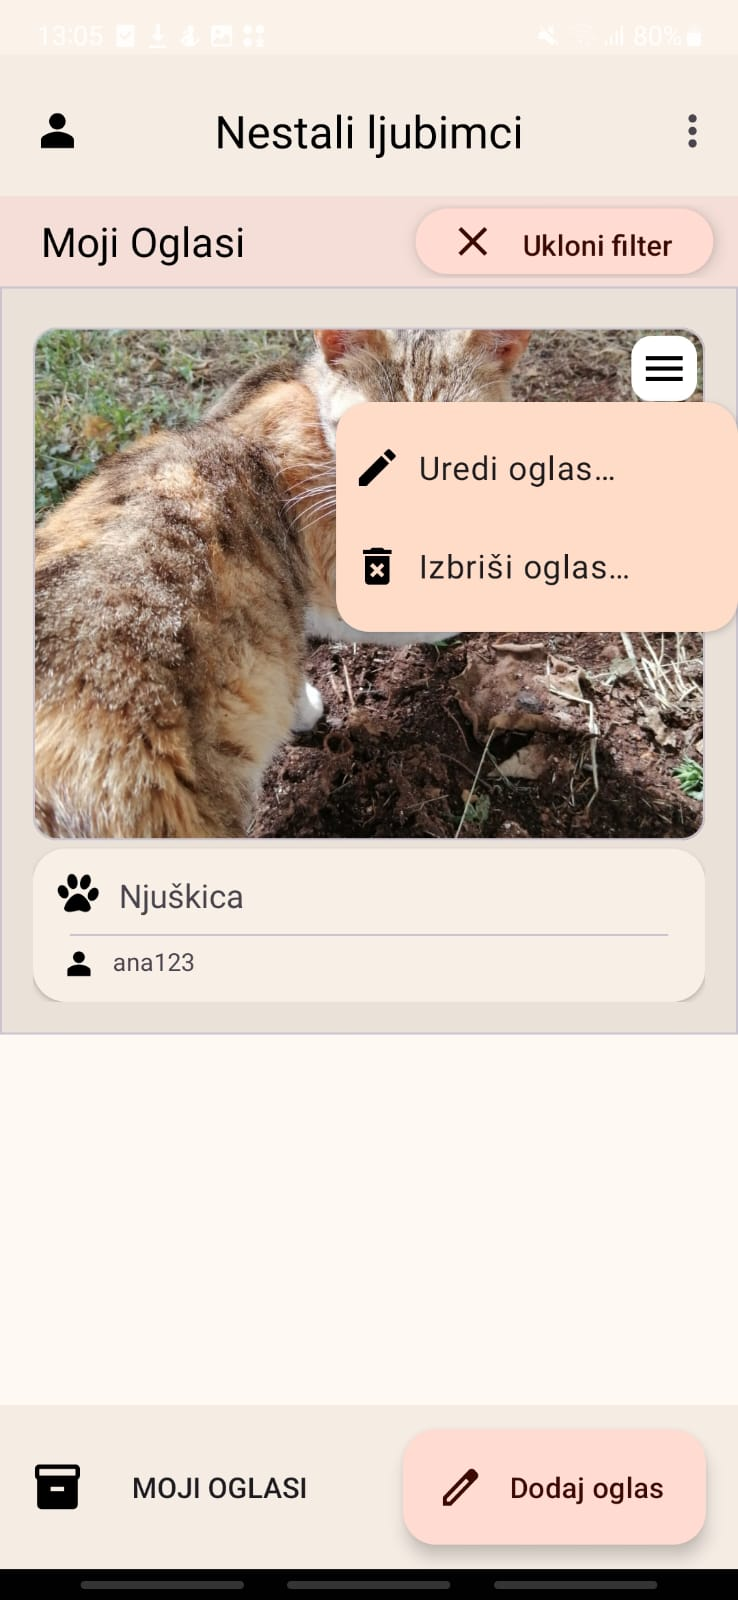
\includegraphics[width=.58\linewidth]{slike/app4v1.jpg}
				  \caption{Odabir brisanja}
				  \label{fig:app4v1}
			\end{minipage}%
			\begin{minipage}{.5\textwidth}
				  \centering
				  
\includegraphics[width=.58\linewidth]{slike/app4v2.jpg}
				  \caption{Potvrda brisanja}
				  \label{fig:app4v2}
			\end{minipage}
			\end{figure}
			\begin{figure}[H]
				  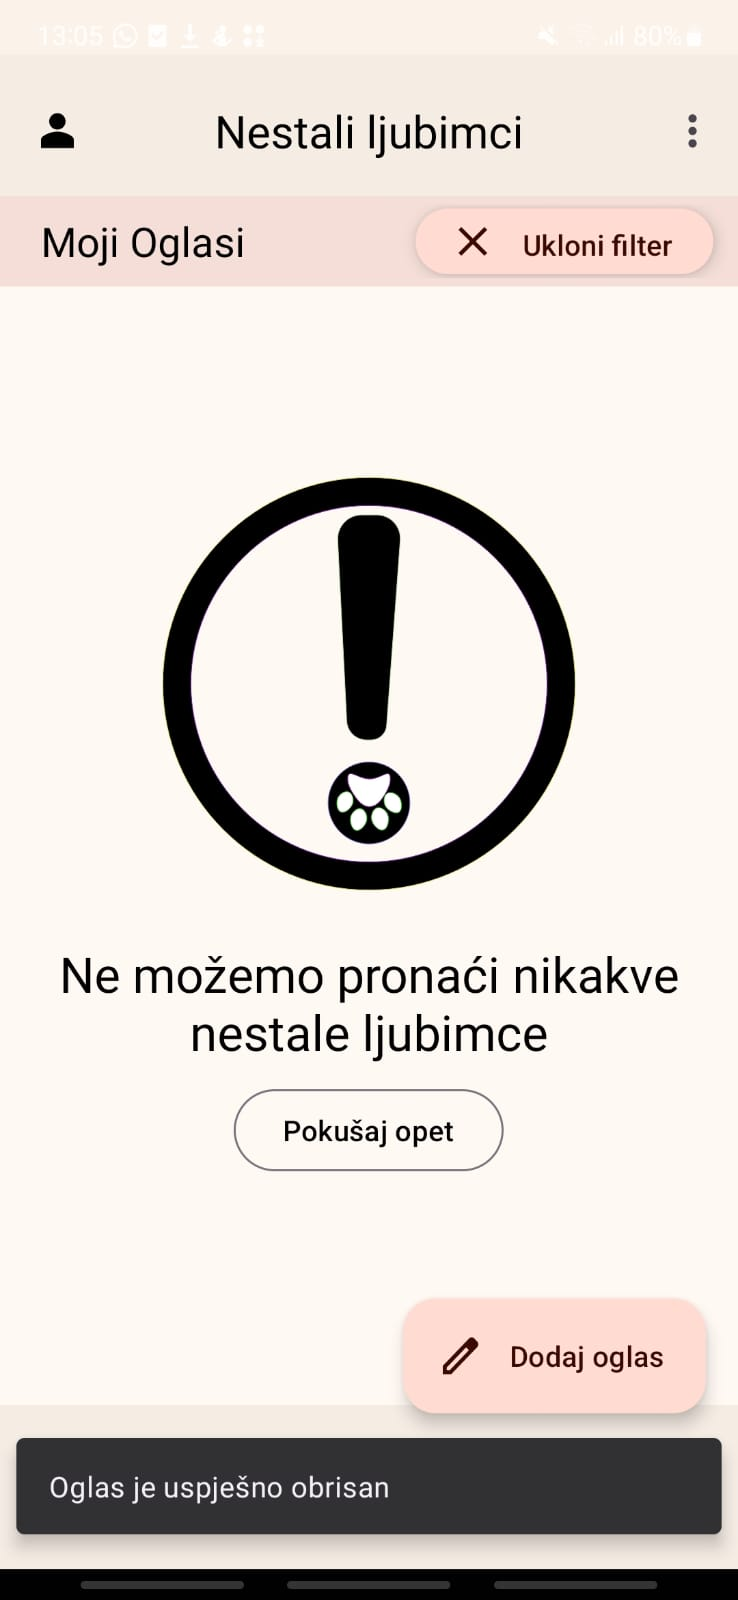
\includegraphics[scale=0.3]{slike/app4v3.jpg}
				  \centering
				  \caption{Prikaz preostalih oglasa}
				  \label{fig:app4v3}
			\end{figure}	 
			
			\eject 
		
		
		\section{Dijagram razmještaja}
			
			UML-dijagrami razmještaja prikazuju fizičku arhitekturu programskog sustava, prikazujući razmještaj programskih artefakata na sklopovskim čvorovima ili virtualnim okruženjima. Arhitektura sustava prepoznaje dvije različite funkcionalnosti - klijenta i poslužitelja. Korisnici pristupaju aplikaciji putem svojih mobilnih uređaja, dok se web poslužitelj i poslužitelj baze podataka nalaze na poslužiteljskom računalu. Komunikacija između korisnika aplikacije i poslužitelja odvija se putem HTTP veze.
			
			 \begin{figure}[H]
			 	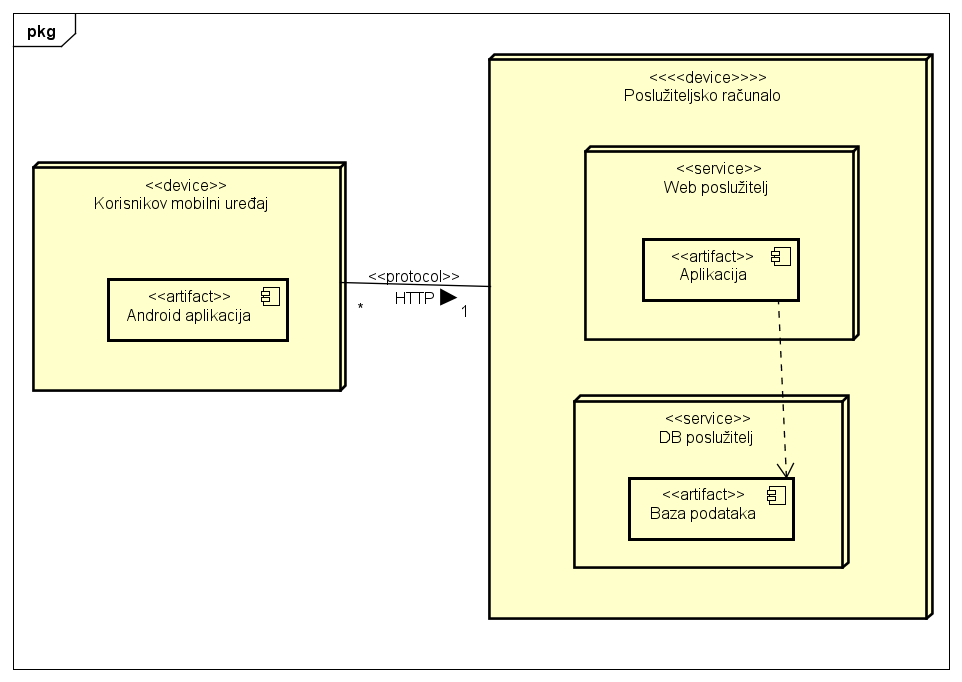
\includegraphics[scale=0.6]{dijagrami/dijagramRazmjestaja/dijagramRazmjestaja.PNG} %veličina slike u odnosu na originalnu datoteku i pozicija slike
			 	\centering
			 	\caption{Dijagram razmještaja}
			 	\label{fig:dRazmjestaja}
			 \end{figure}
			
			\eject 
		
		\section{Upute za puštanje u pogon}
		
		\subsection{Lokalni deploy aplikacije}
		
		\subsubsection{Baza podataka}
		
		Prije pokretanja backend servisa potrebno je lokalno stvoriti bazu podataka. Za to je potreban PostgreSQL poslužitelj baza podataka. Preporučamo dodatno korištenje grafičkih alata kao što su pgAdmin ili DBeaver, ali dovoljan je i samo PostgreSQL driver i konfiguracija iz komandne linije. Upute pratiti na službenim stranicama alata, ovisno o OS-u računala na kojem se pokreće.
		
		Nakon instalacije potrebno je stvoriti bazu podataka. Server očekuje da će se baza zvati „lost\_pets“, ali navedeno se može „pregaziti“ u settings.py fileu u root folderu backenda, u varijabli DEFAULT\_DATABASE. Ipak, preporučujemo da bazu nazovete „lost\_pets“.
		
		Ako se koristi pgAdmin, baza se može stvoriti odabirom „Servers“ $\rightarrow$ „PostgreSQL“ na lijevoj strani ekrana, a zatim desni klik na „PostgreSQL“ pa „Create“ $\rightarrow$ „Database“. Zatim se otvara prozor u kojem se unosi ime baze (\ref{fig:deploy1}) i nakon toga „Save“.
		
		\begin{figure}[H]
			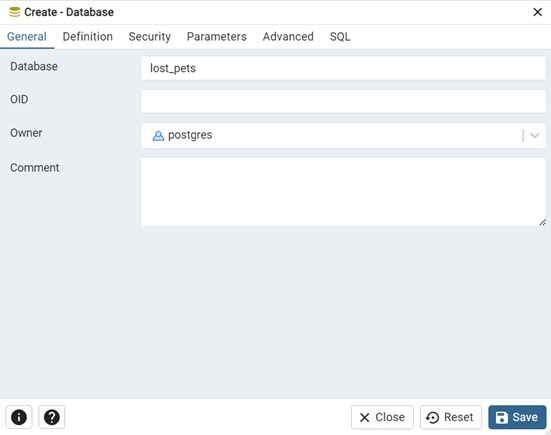
\includegraphics[scale=0.65]{slike/deploy1.jpg} %veličina slike u odnosu na originalnu datoteku i pozicija slike
			\centering
			\caption{Unos imena baze u pgAdminu}
			\label{fig:deploy1}
		\end{figure}
		
		User i password za pristup bazi su konfigurabilni, i preporučujemo mijenjati ih, ako je potrebno, u .env fileu, u varijablama POSTGRES\_USER i POSTGRES\_PASSWORD (Prilagoditi svojim PostgreSQL postavkama). Kako se postgres server defaultno nalazi na portu 5432, a bazu konfiguriramo lokalno, preporučujemo ostaviti POSTGRES\_HOST="localhost" te POSTGRES\_PORT=5432, iako se navedene postavke mogu i mijenjati.
		
		Ove se postavke kod deploya na remote poslužitelj također "pregaze" pomoću varijabli okruženja.
		
		Kada je sve od navedenog postavljeno, baza je spremna za početak rada servera. Tablice stvara repeatable skripta run\_migrations, a početne podatke ubacuje repeatable skripta init\_populate, koje se obje pokreću automatski kod pokretanja servisa.
		
		\subsubsection{Pokretanje servisa}
		
		Najlakši način za deploy servisa jest buildati Docker image iz Dockerfilea, a zatim pokrenuti Docker container iz spomenutog imagea. Ovo osigurava da će server imati sve što mu je potrebno i pokretati se u izoliranom okruženju. Upute za to pratiti na službenim Docker stranicama.
		
		Ovaj će se pristup skoro uvijek koristiti, i automatiziran je, kod deploya na remote server, a za detaljnije upute (poput postavljanja varijabli okruženja objašnjenih prije) potrebno je slijediti upute alata koji pruža usluge poslužitelja.
		
		Ipak, postoji relativno jednostavan način za pokretanje bez buildanja Docker image-a, a to je u virtualnom okruženju, uz lokalni python interpreter. Ukoliko ste na Linuxu, dovoljno će biti izvršiti sljedeće naredbe iz root foldera backenda (folder backend-service):
		
		\begin{lstlisting}
sudo apt-get update
sudo apt-get install python3
sudo apt-get install python3-pip
sudo apt install python3-venv
python3 -m venv ./venv
source venv/bin/activate
pip3 install -r requirements.txt
uvicorn service.main:app \end{lstlisting}

		Na windows OS-u pokretanje je nešto drugačije.
		
		Potrebno je imati instaliran python 3.10 (radi i sa 3.11) i odgovarajući pip installer.
		
		Nakon toga pozicionirati se u root folder backenda (backend-service) u command promptu i pokrenuti slijedno naredbe:
		
		\begin{lstlisting}
python -m venv ./venv
venv\Scripts\activate
pip install -r requirements.txt
uvicorn service.main:app \end{lstlisting}
		
		
		U oba slučaja servis bi se sada trebao nalaziti na http://localhost:8000, a Swagger dokumentacija (popis endpointa i mogućnost slanja direktnog requesta) dostupna je na http://localhost:8000/docs .
		
		\subsection{Postupak izgradnje i objave aplikacije}
		
		\subsubsection{Priprema za objavu}
		\begin{enumerate}
			\item[a)] Odabir ikone aplikacije
			\item[b)] Konfiguracija aplikacije
			
			Konfiguracija aplikacije uključuje: isključivanje debugginga
		\end{enumerate}
		
		\begin{figure}[H]
			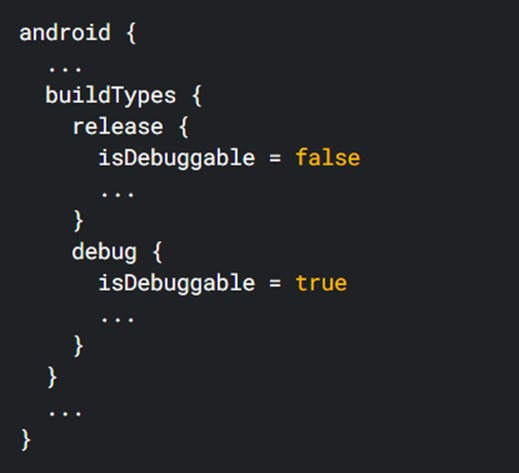
\includegraphics[scale=0.6]{slike/deploy2.jpg} %veličina slike u odnosu na originalnu datoteku i pozicija slike
			\centering
			\caption{Isključivanje logiranja, pregleda android manifesta te build opcija, odabir odgovarajučeg ID-a aplikacije.}
			\label{fig:deploy2}
		\end{figure}
		
		\subsubsection{Postavljanje verzije}
		
		\begin{figure}[H]
			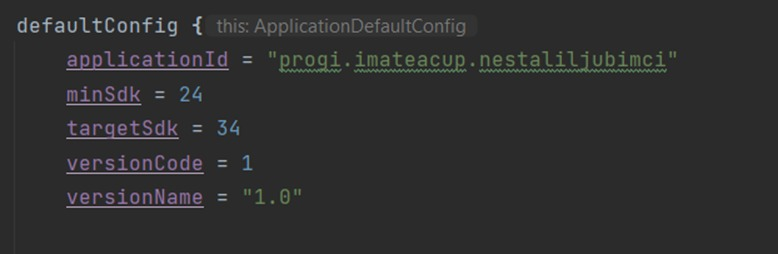
\includegraphics[scale=0.5]{slike/deploy3.jpg} %veličina slike u odnosu na originalnu datoteku i pozicija slike
			\centering
			\caption{Postavljanje verzije}
			\label{fig:deploy3}
		\end{figure}
		
		\subsubsection{Potpis aplikacije i release build aplikacije}
		
		Potrebno je generirati upload key i keystore, što je moguće korištenjem alata Android Studio.
		
		Nakon što je keystore generiran, moguće je izgraditi release verziju aplikacije u .aab ili .apk formatu. U Android Studiu odabrati \texttt{Build -> Select Build Variant} i odabrati "release". Zatim \texttt{Build -> Generate Signed Bundle(s) / Apk}, odabrati, u našem slučaju, APK.
		
		\begin{figure}[H]
			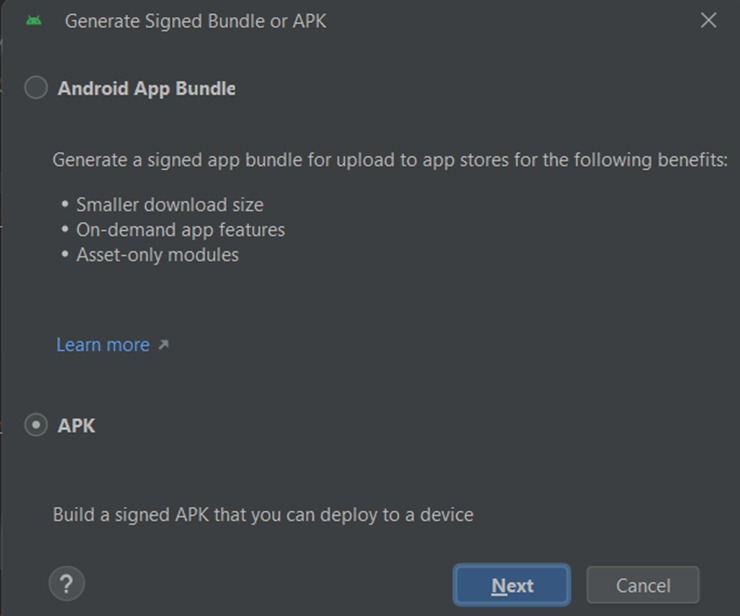
\includegraphics[scale=0.45]{slike/deploy4.jpg} %veličina slike u odnosu na originalnu datoteku i pozicija slike
			\centering
			\caption{Odabir APK}
			\label{fig:deploy4}
		\end{figure}
		
		Stisnuti \texttt{Next}, odabrati \texttt{key store path} koji vodi na ranije generirani keystore i unjeti \texttt{keystore}, \texttt{key password} i \texttt{alias}.
		
		\begin{figure}[H]
			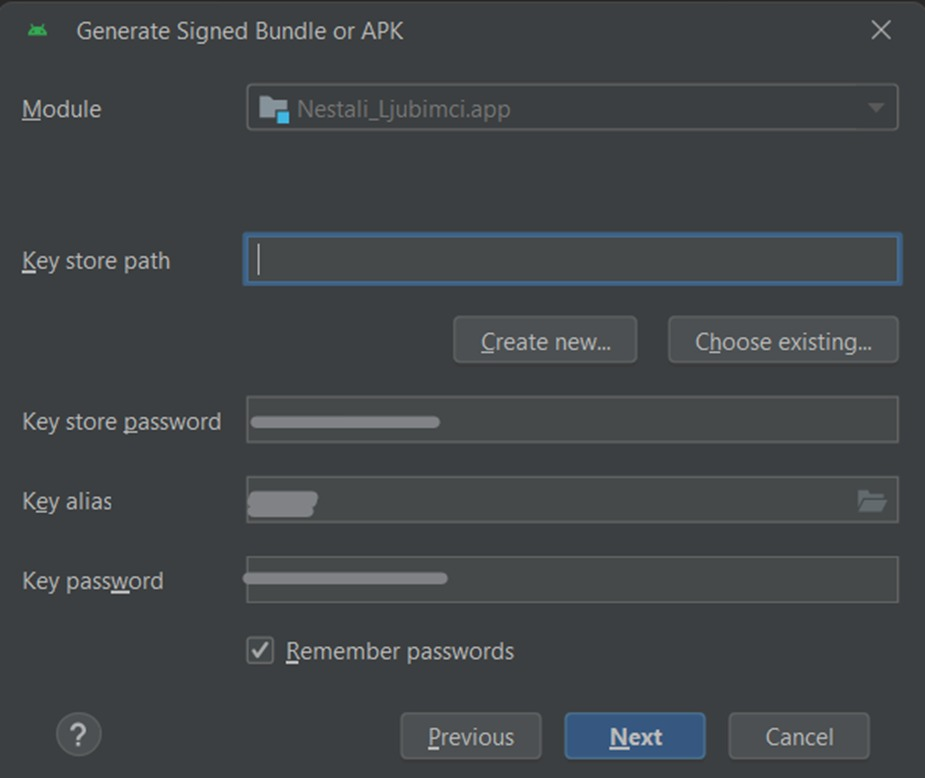
\includegraphics[scale=0.3]{slike/deploy5.jpg} %veličina slike u odnosu na originalnu datoteku i pozicija slike
			\centering
			\caption{Unos za keystore, key password i allias}
			\label{fig:deploy5}
		\end{figure}
		
		Stisnuti \texttt{Next}, odabrati \texttt{build variant}, odredišni folder i kliknuti \texttt{Create}. Potpisani APK će se nalaziti u specificiranom folderu.
		
		\begin{figure}[H]
			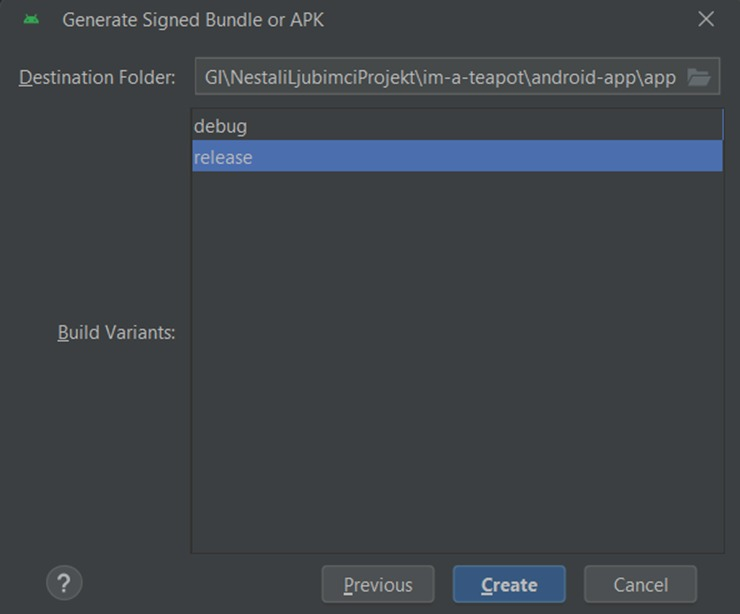
\includegraphics[scale=0.43]{slike/deploy6.jpg} %veličina slike u odnosu na originalnu datoteku i pozicija slike
			\centering
			\caption{Odabir mape za APK i izrada}
			\label{fig:deploy6}
		\end{figure}
		
		\subsubsection{Objava aplikacije na odabranom appstore-u}
		
		Objava aplikacije znatno se razlikuje na različitim trgovinama aplikacija, a postupak objave često je rigorozan te se nerijetko plaća. Zbog takve kompleksnosti i spomenutih razlika u procesu objave, nećemo ulaziti u detalje već ćemo ukratko opisati postupak objave na Amazon Appstoreu.
		
		Za početak, potrebno je napraviti račun na Amazon Appstoreu te se navigirati na sljedeću stranicu: \sloppy\url{https://developer.amazon.com/docs/app-submission/submitting-apps-to-amazon-appstore.html}.
		
		Prateći upute na priloženoj stranici, potrebno se ulogirati u Amazon Developer konzolu. Zatim kliknuti na \textit{dashboard} te nakon toga odabrati \textit{Add a New App} iz padajućeg izbornika i odabrati \textit{Android}. Ponovno odabrati \textit{Add a New App} te \textit{Android}. Zatim je potrebno pratiti formu te ispuniti sva polja koja Amazon zahtijeva te generirati zahtjev za objavu. Nakon što se to uspješno obavi, potrebno je čekati da Amazon Appstore odobri upload aplikacije.
		
		
		\eject
		